\documentclass[a4paper]{easychair}

\newcommand{\easychair}{\textsf{easychair}}

% This provides the \BibTeX macro
\usepackage{doc}
% \usepackage{makeidx}

% If you plan on including some algorithm specification, we recommend
% the below package. Read more details on the custom options of the
% package documentation.
%
% \usepackage{algorithm2e}

%\makeindex

%% Document
%%
\begin{document}

%% Front Matter
%%
% Regular title as in the article class.
%
\title{Project Group\\ Applied Functional Programming\\
       \large{Web Development with Haskell}}

% \titlerunning{} has to be set to either the main title or its shorter
% version for the running heads. When processed by
% EasyChair, this command is mandatory: a document without \titlerunning
% will be rejected by EasyChair

\titlerunning{Web Development with Haskell}

% Authors are joined by \and. Their affiliations are given by \inst, which indexes
% into the list defined using \institute
%
\author{
  Meike Grewing
\and
  Lukas Heidemann
\and
  Fabian Thorand
\and 
  Fabian Zaiser\\
}

% Institutes for affiliations are also joined by \and,
\institute{
  Informatik, Universit\"at Bonn,
  Germany
\\
 }
%  \authorrunning{} has to be set for the shorter version of the authors' names;
% otherwise a warning will be rendered in the running heads. When processed by
% EasyChair, this command is mandatory: a document without \authorrunning
% will be rejected by EasyChair

\authorrunning{Grewing, Heidemann, Thorand, Zaiser}


\clearpage

%%%%%%%%%%%%%%%%%%%%%%%%%%%%%%%%%%%%%%%%%%%%%%%%%%%
\maketitle
%%%%%%%%%%%%%%%%%%%%%%%%%%%%%%%%%%%%%%%%%%%%%%%%%%%

\begin{abstract}
The goal of the project group ``Applied Functional Programming'' was to get an insight into web development using Haskell and the web framework \emph{Yesod}. 
In this paper, we want to document our main project, a web implementation of the well-known game \emph{Battleships}. You can find the code on GitHub\footnote{\url{https://github.com/zrho/afp/tree/master/battleships}} and play the current production version\footnote{\url{http://www-pg.iai.uni-bonn.de/battleships}}.
\end{abstract}

\setcounter{tocdepth}{2}

\pagestyle{empty}


%------------------------------------------------------------------------------
\section{Introduction}
\label{sect:intro}
Our main project was to develop a \emph{Battleships} web application providing a neat graphical user interface and an adjustable AI to play against.
We decided to use the following rules:
\begin{itemize}
 \item Each player begins with a total of ten ships: one ship of length five, two of length four, three of length three and four of length two.

 \item When a shot hit a ship, the player may fire again.
\end{itemize}

In addition to the usual rules, our version of the game includes some modifications:

\begin{itemize}
 \item 
 In addition to firing a shot, the player is allowed to move one of his ships forward or backward by one cell in each round (adhering to the placement regulations).
 \item
 As soon as one of your ships is completely sunk, other ships can be moved across the space it previously occupied.
 \item
 The number of turns is limited to prevent endless games. After the last turn, the player with the most remaining ships wins.
\end{itemize}

\begin{figure}
 \centering
  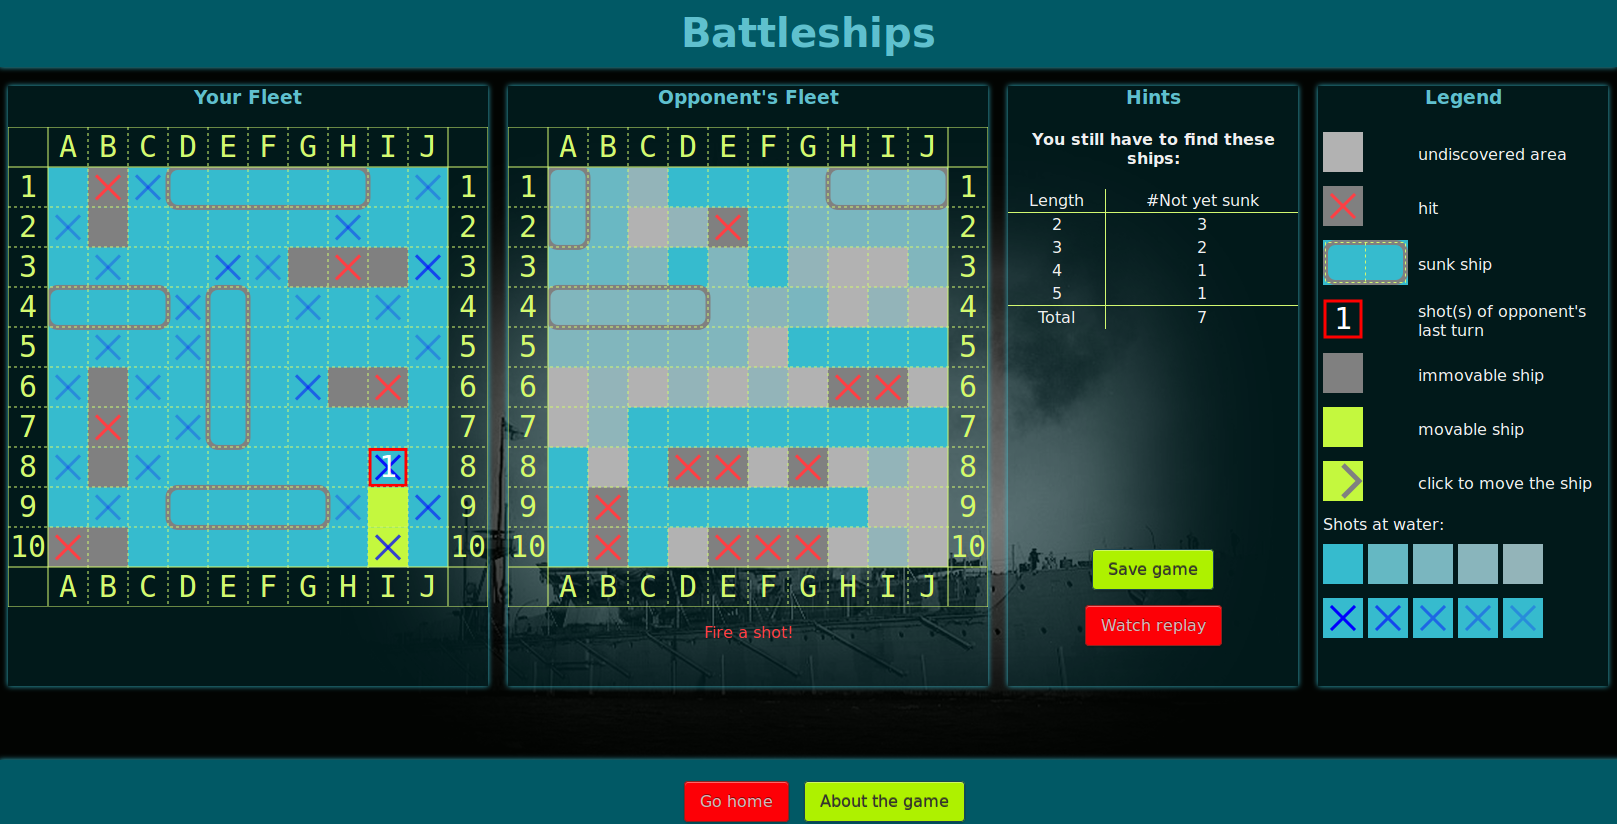
\includegraphics[width=\textwidth]{play.png}
 \caption{Typical game view. Shots are fired by clicking on the target.}
\end{figure}

\begin{figure}
 \centering
  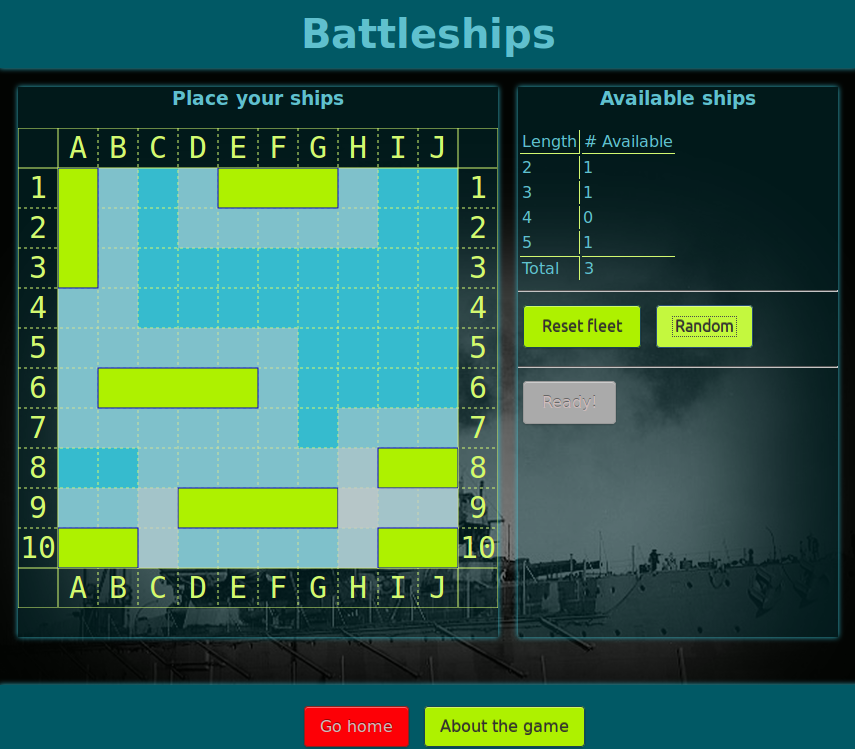
\includegraphics[scale=0.25]{place.png}
 \caption{The ships can be placed randomly or via drag and drop.}
\end{figure}

\begin{figure}
 \centering
  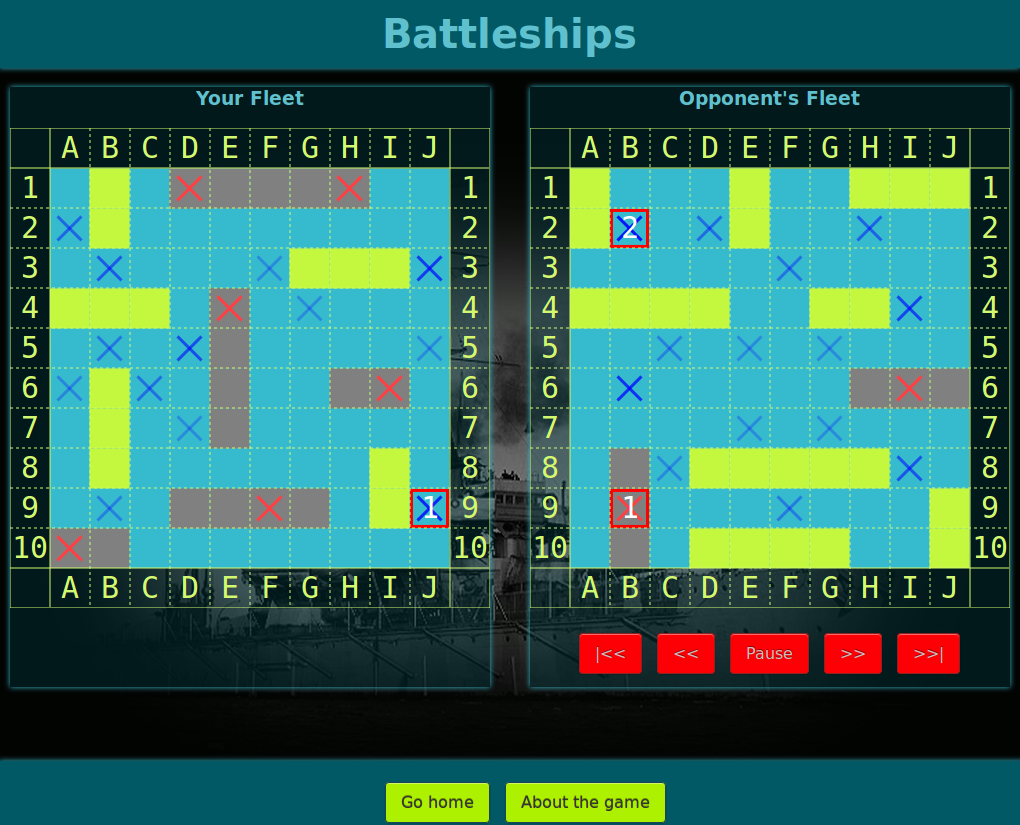
\includegraphics[scale=0.25]{replay.png}
 \caption{Recap of the game. (animated)}
\end{figure}

%-----------------------------------------------------------------------------
\section{Architecture and Framework}

For our project, we used the \emph{Yesod} Web Framework\footnote{\url{http://www.yesodweb.com/}} developed by Michael Snoyman and others. Its goals are performance, type-safety and conciseness of code.

For these purposes Yesod offers embedded DSLs\footnotetext{Domain Specific Languages} for writing HTML, CSS and Javascript code which allow using variables from Haskell code and are syntactically simpler (e.g. the DSL for HTML uses indentation instead of closing tags). There is also a lot of compile-time checking involved. For example, URLs in Yesod are type safe, meaning that one specifies which parameters a certain route expects and their types. Whenever it is referenced, e.g. in hyperlinks or redirections, the compiler checks if the expected and actual data formats match. This makes 404 errors for internal links almost impossible. Yesod also offers good support for internationalization. In fact, our project web site is available in English and German.

The game logic resides on the server and is completely written in Haskell. On the client side, we use JavaScript for ship placement, handling of clicks on the boards and viewing the replay. The game state is not stored on the server but is sent back and forth between client and server. To prevent manipulations on the client side, the state is encrypted before being exposed. %% TODO: explain why we did that.

%-----------------------------------------------------------------------------
\section{Demonstrating that the AI Plays Fair}
\label{sect:fair-play}
Of course, the AI should play fair and observe the same rules as the human player. Allowing ship movement makes it hard to check the AI for fair play by just playing, so we tried our best to clarify that the AI cannot ``cheat'':

\begin{itemize}
 \item After the game ends, we produce an animated recap of the course of the game to help the player comprehend what happened at what time. 
 \item We use Haskell's type system to make it easy to find the places in the code where the AI does get information and interact with the game logic. This way, it is easier to check the code to convince oneself that the the AI cannot cheat.
 
 %% The following 2 paragraphs are probably too detailed ... But shouldn't we at least mention some of Haskell's features?

 More precisely, every AI is an instance of the type class\footnote{Type classes in Haskell correspond very roughly to interfaces in OOP} \verb+AI+ which has to implement the four functions \verb+aiInit+ (initializing the AI), \verb+aiFire+ (computing the next target of the AI), \verb+aiResponse+ (giving the AI feedback about its last target) and \verb+aiMove+ (computing which ship the AI moves).
 
 For instance, the type signature of \verb+aiFire+ looks like this:
 \begin{verbatim}
  aiFire :: (MonadRandom m, MonadState ai m) => m Pos
 \end{verbatim}
 This means that the function is executed in a context that allows non-determinism (\verb|MonadRandom|) and access to the AI's state (\verb|MonadState|) and that it returns a position (\verb|Pos|) which it wants to target. Thanks to Haskell's type system, it can't have any other side effects (IO etc.). The game handling code is polymorphic in the AI type, so it can only interact with the AI via these functions. Thus it is easy to verify that the AI doesn't receive additional information: One only needs to look at the places where the four aforementioned functions are invoked.

\end{itemize}

%------------------------------------------------------------------------------
\section{Battleships AI}
\label{sect:battleships-ai}
In addition to a simple AI which basically does everything at random, we implemented a much more sophisticated AI which we are going to describe in some detail here.

\subsection{Blocked Cells}
When deciding on a cell to fire at, it is necessary to know which cells cannot currently be occupied by a ship. We call these cells \emph{blocked}. 
We draw our information about blocked cells from the following situations:
\begin{itemize}
 \item 
 If we just found out that at a certain position there is water, that position is blocked.
 \item
 If we just sunk a ship, all its cells are blocked. This includes its \emph{safety margin} (ships cannot touch, so cells directly around a ship cannot be occupied by any other ship).
 \item 
 If the cell is diagonally adjacent to a cell that was a successful hit, it is blocked because of the hit ship's safety margin.
\end{itemize}

\subsection{Probabilities}
When ships are movable, you often cannot tell for sure whether a cell is blocked or not. Thus, we need to work with probabilities. When the AI just hit water the probability for this cell to be water is 1. Over time, however, this probability declines. The decline is modeled as exponential decay with factor 0.98. This means that one shot later the water probability for the cell is 0.98, then 0.96, then 0.941 etc. The same decline is applied to the cells blocked because of a sunk ship, because right after being sunk other ships can start moving across it.

\subsection{Scoring}
The AI selects its next target by computing a \emph{score} for each position. A high score indicates a high probability to hit a ship at that position, so the AI chooses the position with the highest score as its next target. To make playing more interesting, we added some randomness to calculating the scores. The amount of randomness depends on the selected difficulty level; the scoring method depends on whether ships are movable or not.

\subsubsection{Immovable Ships} Given a position to score, the AI considers all potential ships that this position is part of. These are weighted according to the probabilities computed before. Also, if a ship is hit or will be sunk in the next move according to the AI's tracking information, it is given an extra high score, because this ship is very likely to exist.

Note that the AI does not consider and weight whole fleets according to the probabilities, but only does this locally for each position. So it might happen that a position gets a positive score although it would be ruled out if the AI were testing whole fleets instead of individual ships.

Then the AI applies a checkerboard pattern, i.e. multiplies half of the scores by 0.9, so it won't have to hit all cells to find all ships. Positions at the edge of the board naturally allow fewer ships to pass through them. But the AI shouldn't be biased towards the center, so the scores are divided by the scores at the beginning of the game. If we already attacked that position before, its score is 0.

\subsubsection{Movable Ships} In this case there are 2 phases because of the limited amount of turns: As the timeout approaches, the AI changes its strategy to win after timeout. 
\begin{description}
 \item[Search Phase] 
 This is what the AI does in the beginning. It strictly follows a checkerboard pattern to find (and not sink!) all ships. Sinking is not beneficial at this stage because it allows ships to move around more freely. Also, hit ships get score 0, because the primary goal is to find all ships and not to hit the already found ones.
 \item[Sink Phase] 
 When the AI has hit enough ships (or if the countdown towards the end of the game is running), we move on to the 2nd phase. Currently ``enough ships'' means that the number of hits is at least half the number of cells occupied by the remaining ships. This is the minimum number of hits needed when we want all ships to be hit wherever the checkerboard pattern allows it.
\end{description}
In the second phase, now that we've hopefully found all ships, our strategy is essentially the same as in the immovable case. We just don't use the checkerboard pattern any longer because that was already used extensively in phase 1 and we have to hit all parts of a ship to sink it.


\subsection{Moving Ships}
In each turn, the AI generates all possible movements of all movable ships and chooses one at random, or -- also randomly -- decides not to move at all. %Todo: Sounds a little strange, maybe we should elaborate on this?

%------------------------------------------------------------------------------
% Refs:
%
\label{sect:bib}
\bibliographystyle{plain}
%\bibliographystyle{alpha}
%\bibliographystyle{unsrt}
%\bibliographystyle{abbrv}
%\bibliography{easychair}

%------------------------------------------------------------------------------
% Index
%\printindex

%------------------------------------------------------------------------------
\end{document}

% EOF
